% Preamble ==================================================================
\documentclass[11pt]{article}
\usepackage{geometry}
\geometry{verbose,tmargin=2.5cm,bottom= 1.5cm,lmargin=2.5cm,rmargin=2.5cm}
\usepackage{float}
\usepackage{graphicx}
\usepackage{amsmath}
\usepackage{amssymb}
\usepackage{enumitem}
\usepackage{mathtools}

\usepackage{amsthm} % theorem
\usepackage{listings} % code snippets
\usepackage{fancyvrb} %verbatim
\lstset{frame=l,
  language=Python,
  basicstyle={\small\ttfamily},
  numbers=none,
  numberstyle=\tiny\color{black},
  keywordstyle=\color{black},
  commentstyle=\color{blue},
  stringstyle=\color{mauve},
}

\numberwithin{equation}{section}

\usepackage{titlesec,dsfont}

%Format section heading style
\usepackage{sectsty}
\sectionfont{\sffamily\bfseries\large}
\subsectionfont{\sffamily\normalsize\slshape}
\subsubsectionfont{\sffamily\small\itshape}
\paragraphfont{\sffamily\small\textbf}


%Put period after section number
\makeatletter
\def\@seccntformat#1{\csname the#1\endcsname.\quad}
\makeatother

%Bibliography
\usepackage[round]{natbib}
\bibliographystyle{genetics}

%Format captions
\usepackage[ labelsep=period, justification=raggedright, margin=10pt,font={small},labelfont={small,normal,bf,sf}]{caption}

\setlength{\parskip}{0ex} %No space between paragraphs.

\renewcommand{\familydefault}{\sfdefault}

\newcommand\indep{\protect\mathpalette{\protect\independenT}{\perp}}
\newcommand{\nindep}{\not\!\perp\!\!\!\perp}
\def\independenT#1#2{\mathrel{\rlap{$#1#2$}\mkern2mu{#1#2}}}

%PUT ME LAST--------------------------------------------------
\usepackage[colorlinks=true
,urlcolor=blue
,anchorcolor=blue
,citecolor=blue
,filecolor=blue
,linkcolor=black
,menucolor=blue
,linktocpage=true
,pdfproducer=medialab
,pdfa=true
]{hyperref}

\makeatother %Put this last of all


\newcommand{\defeq}{\coloneqq}
\newcommand{\overbar}[1]{\mkern 1.5mu\overline{\mkern-1.5mu#1\mkern-1.5mu}\mkern 1.5mu}

% Make theorems bold
\makeatletter
\def\th@plain{%
  \thm@notefont{}% same as heading font
  \itshape % body font
}
\def\th@definition{%
  \thm@notefont{}% same as heading font
  \normalfont % body font
}
\makeatother

\newtheorem{thm}{Theorem}[section]
\newtheorem{defn}{Definition}[section]
\newtheorem{cor}{Corollary}[section]
\newtheorem{prop}{Property}[section]
\newtheorem{rle}{Rule}[section]
\newtheorem{lma}{Lemma}[section]

%Preamble end--------------------------------------------------


\begin{document}

\begin{flushleft}
\textbf{\Large Sequence models}
\end{flushleft}

\begin{flushleft}
Author: Juvid Aryaman

Last compiled: \today
\end{flushleft}

\noindent This document contains my personal notes on sequence models.


\section{Embeddings}
Embeddings are tensors. You interact with that tensor by indexing into it. It is often used to store encodings of collections of words. For example:
\begin{lstlisting}
>>> nn.Embedding(vocab_sz, n_hidden)
\end{lstlisting}	
creates a set of \verb#vocab_sz# tensors, each of size \verb#n_hidden#. 

A common thing to do is to something like:
\begin{lstlisting}
>>> embedding = nn.Embedding(10, 3)
>>> input = torch.LongTensor([[1,2,4,5],[4,3,2,9]])
>>> embedding(input)

tensor([[[-0.0251, -1.6902,  0.7172],
         [-0.6431,  0.0748,  0.6969],
         [ 1.4970,  1.3448, -0.9685],
         [-0.3677, -2.7265, -0.1685]],

        [[ 1.4970,  1.3448, -0.9685],
         [ 0.4362, -0.4004,  0.9400],
         [-0.6431,  0.0748,  0.6969],
         [ 0.9124, -2.3616,  1.1151]]])
\end{lstlisting}
so you can see that the input is \verb#[sentence1, sentence2]#, where sentence 1 consists of words \verb#[1,2,4,5]#. As an output, we get the corresponding 3-vectors for each word. So the output is: 
\begin{lstlisting}
[[[embedding_word_1,   # length 3 vector
   embedding_word_2, 
   embedding_word_4, 
   embedding_word_5],
  
  [embedding_word_4, 
   embedding_word_3, 
   embedding_word_2, 
   embedding_word_9]
]]
\end{lstlisting}

\section{Linear layer}
Applies a linear transformation to the incoming data: $y = xA^T + b$
\begin{lstlisting}
>>> m = nn.Linear(20, 30)
>>> input = torch.randn(128, 20)
>>> output = m(input)
>>> print(output.size())
torch.Size([128, 30])
\end{lstlisting}


\section{Recurrent neural network}
Torch, by default, applies a multi-layer Elman RNN. This is defined as applying the following function to each element of the input sequence
\begin{align}
h_t  &= \sigma_h(W_h x_t + U_h h_{t-1} + b_h)\\
y_t  &= \sigma_y(W_y h_t + b_y)
\end{align}
where $x_t$ is an input vector, $h_t$ is a hidden layer vector, $y_t$ is an output vector, $W, U, b$ are parameter matrices and vector, $\sigma_h, \sigma_y$ are activation functions. Note that we don't actually retain the hidden state between lines -- we throw it away after every complete training example (a line). We will typically initialize the hidden state to be $h_{t=0}=0$. Within a particular training instance, on a particular line, we may have different maximum values of $t=T$. 

For example, in word classification, where we construct a character-level RNN, in each training loop we will
\begin{enumerate}[noitemsep]
\item Get an input and target tensor
\item Create a zeroed initial hidden state
\item Read each letter in and:
\begin{itemize}[noitemsep]
\item Keep hidden state for next letter
\item Feed the previous hidden state $h_{t-1}$ in with the current input $x_t$
\end{itemize}
\item Compare output at the end of the RNN loop to the target
\item Back-propagate
\end{enumerate}
Then return the output and loss.

\begin{figure}
\begin{center}
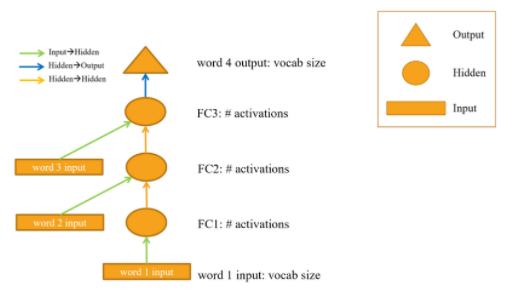
\includegraphics[width=0.8\columnwidth]{../figures/rnn.png}  
\end{center}
\caption{Graphical representation of RNN
}
\label{fig:rnn}
\end{figure}

\subsection{Gated recurrent unit}
A GRU is a type of RNN. They are similar to LSTMs but have fewer parameters and can be easier to train. The key innovation is that they allow the network to control the amount of information which flows between consecutive time steps, and allows the network to forget. 

For each element in the input sequence, each layer computes the following function:
\begin{align}
z_t &= \sigma(W_{iz}x_t + b_{iz} + W_{hz} h_{(t-1)} + b_{hz}) \label{eq:gru_update_gate_zt} \\
r_t &= \sigma(W_{ir}x_t + b_{ir} + W_{hr}h_{(t-1)} + b_{hr}) \label{eq:gru_reset_gate_rt} \\
n_t &= \tanh(W_{in} x_t + b_{in} + r_t \odot (W_{hn} h_{(t-1)} + b_{hn}) ) \label{eq:gru_candidate_hidden_state_nt} \\
h_t &= (1-z_t) \odot n_t + z_t \odot h_{(t-1)} \label{eq:update_ht}
\end{align}
where $x_t$ is the input at time $t$, $h_t$ is the hidden state at time $t$. $r_t$, $z_t$, and $n_t$ are the reset, update, and new gates respectively. $\sigma$ is the sigmoid function, and $\odot$ is the Hadamard product.

\begin{figure}
\begin{center}
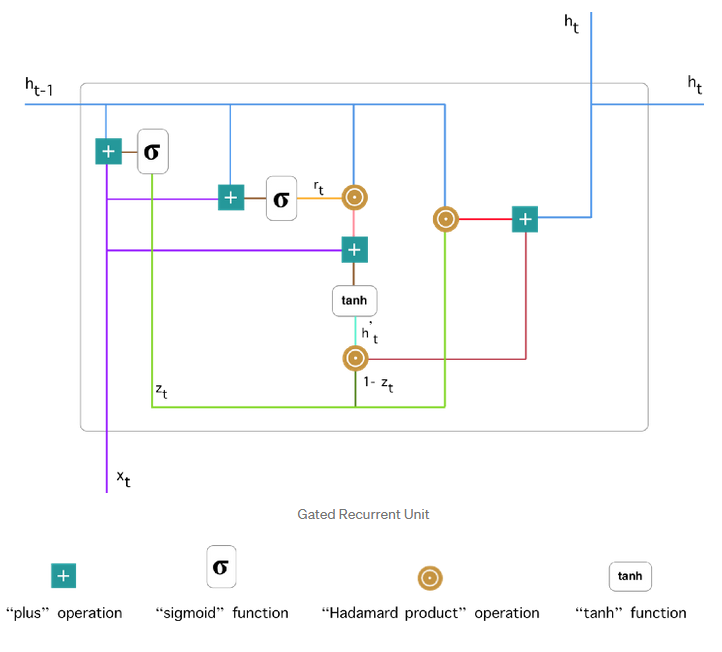
\includegraphics[width=0.8\columnwidth]{../figures/gru.png}  
\end{center}
\caption{Graphical representation of GRU. I don't actually find these super-helpful.
}
\label{fig:rnn}
\end{figure}

\begin{enumerate}[noitemsep]
\item Eq.\eqref{eq:gru_update_gate_zt} is called the \textbf{update gate}. The update gate combines the input with the previous hidden state. It determines how much of the previous step's hidden state $h_{t-1}$ is passed onto the new hidden state $h_{t}$ in Eq.\eqref{eq:update_ht}.
\item Eq.\eqref{eq:gru_reset_gate_rt} is called the \textbf{reset gate}. The formula is the same as Eq.\eqref{eq:gru_update_gate_zt}. It will be used to decide how much of the past information to \textbf{forget} in Eq.\eqref{eq:gru_candidate_hidden_state_nt}.
\item Eq.\eqref{eq:gru_candidate_hidden_state_nt} is a \textbf{candidate} hidden state. It combines the current input with some weighting of the previous hidden state. The reset gate $r_t$ has an element-wise product with $h_{t-1}$, allowing the network to forget $h_{t-1}$ as $r_t \rightarrow 0$. 
\item Eq.\eqref{eq:update_ht} mixes the previous hidden state $h_{t-1}$ with the candidate hidden state $n_t$ through a convex combination weighted by $z_t$.
\end{enumerate}

\section{Attention}
\subsection{Bahdanau attention}
\cite{bahdanau14} were the first to describe an attention model in the context of an encoder-decoder recurrent model. The model is broadly as follows. An encoder reads an input sequence of vectors $x=(x_1,...,x_{T_x})$, where each element corresponds to e.g. a word in a sentence and the vector is an embedding vector with some fixed embedding dimension. They use an RNN to generate a hidden state $h_t \in \mathbb{R}^n$ for each time $t$
\begin{equation}
h_t = f(x_t, h_{t-1})
\end{equation}
and a context vector which, in general, is written as
$c = q(\{h_1,...,h_{T_x}\})$
where both $f$ and $q$ are some non-linear functions. We concatenate the forwards and backwards hidden states of a bidirectional GRU in \verb#seq.enc_dec_attn# to form $c$, see Fig.~\ref{fig:bah-attn}.

\begin{figure}
\begin{center}
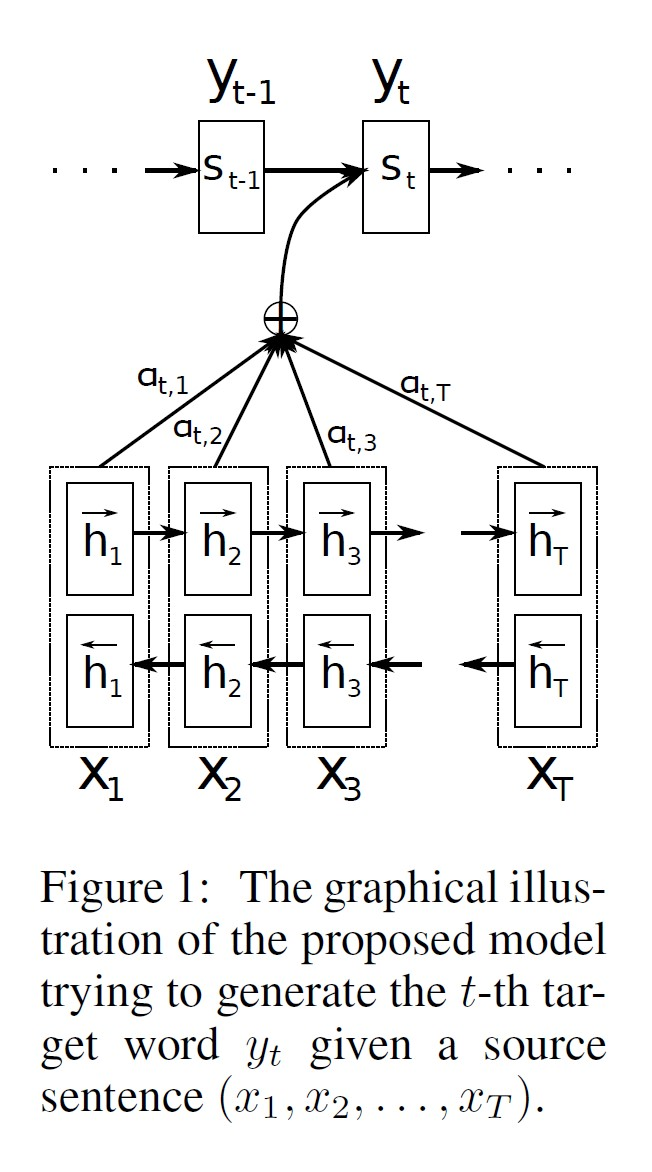
\includegraphics[width=0.4\columnwidth]{../figures/enc-dec-attn.jpg}  
\end{center}
\caption{Bahdanau attention \citep{bahdanau14}, depicting Eq.\eqref{eq:bah-dec-hidden} and Eq.\eqref{eq:bah-attn-mech} graphically.}
\label{fig:bah-attn}
\end{figure}

For the decoder, we have a sequence of target vectors $y=(y_1,...,y_{T_y})$ and an RNN hidden state $s_i$ where
\begin{equation}
s_i = f(s_{i-1}, y_{i-1}, c_i). \label{eq:bah-dec-hidden}
\end{equation}
Notice that, unlike the encoder RNN, the decoder RNN is conditioned on a distinct context vector $c_i$ for each target word $y_i$.

The context vector $c_i$ depends upon the full sequence of encoder hidden states $(h_1, ..., h_{T_x})$, where each of these `annotations' contains information about the whole input sequence but with a strong focus on the parts surrounding the $i$-th word. The context vector is computed using an \textbf{attention mechanism}
\begin{equation}
c_i = \sum_{j=1}^{T_x} \alpha_{ij} h_j \label{eq:bah-attn-mech}
\end{equation}
where $\alpha_{ij}$ is an \textbf{attention probability}. In this equation, $h_j$ is commonly referred to as a ``\textbf{value}'' ($V$), as it is the quantity being reweighted by an attention mechanism ($\alpha$). The attention probability is defined by
\begin{equation}
\alpha_{ij} = \text{softmax}\left( e_{ij} \right) = \frac{\exp(e_{ij})}{\sum_{k=1}^{T_x}\exp(e_{ik})}
\end{equation}
where $e_{ij}$ is an \textbf{attention energy} defined by an \textbf{alignment model}
\begin{equation}
e_{ij} = a(s_{i-1}, h_j) = v_a^T \tanh(W_a s_{i-1} + U_a h_j)
\end{equation}
where $W_a \in \mathbb{R}^{n \times n}$, $U_a \in \mathbb{R}^{n \times 2n}$ and $v_a \in \mathbb{R}^n$. $W_a s_{i-1}$ is commonly referred to as a ``\textbf{query}'' ($Q$), as $s_{i-1}$ is the information being used to look up which of the encoder states to combine with. $U_a h_j$ is referred to as the ``\textbf{key}'' ($K$) -- which is the quantity being reweighted.

The alignment models scores how well the inputs around position $j$ and the output at position $j$ match. The context vector for output position $j$ is therefore a reweighting of the input sequence annotations, according to the `probability' that a particular input is `relevant' for the current output position $j$. See \verb#seq.enc_dec_attn# for an implementation.

\subsection{Scaled dot product attention} \label{sec:dp-attn}
Scaled dot product attention is a slightly simpler approach to attention than Bahdanau attention. We simply pack together a set of $n$ queries, keys, and values into matrices $Q$, $K$, and $V$ respectively. We then compute the function
\begin{equation}
\text{Attention}(Q, K, V) = \text{softmax}\left( \frac{QK^T}{\sqrt{d_k}} \right) V
\end{equation}
where $Q, K \in \mathbb{R}^{n \times d_k}$ and $V \in \mathbb{R}^{n \times d_v}$. The factor of $\sqrt{d_k}$ attempts to reduce the variance of the dot product, and therefore keep the softmax function in regions of non-negligible gradient.

\newcommand{\dmodel}{d_{\text{model}}}

\section{Transformers}


\subsection{Embedding}
Transformers \citep{Vaswani17} use regular-old embeddings for the source and target (see Fig.~\ref{fig:tfm}). The embedding dimension is $\dmodel$.

\begin{figure}
\begin{center}
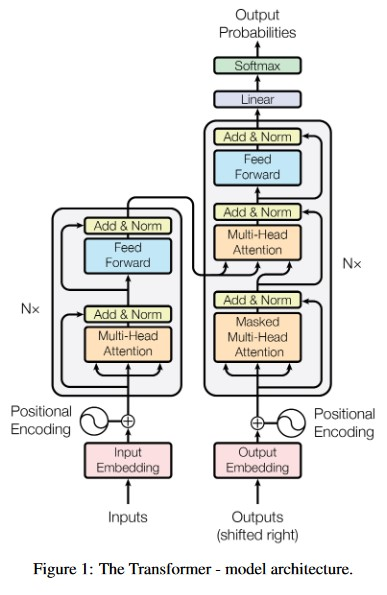
\includegraphics[width=0.4\columnwidth]{../figures/transformer.jpg}  
\end{center}
\caption{The infamous transformer diagram.}
\label{fig:tfm}
\end{figure}

\newcommand{\demb}{d_{\text{emb}}}
\subsection{Positional encoding}
After generating the embeddings, we \textbf{add} a different sinusoidal function to each dimension of the embedding $\demb$, where the sinusoid is continuous along the sequence length of the input (namely either the source or target). Doing this gives the input positional information, which is necessary as there are no recurrent or convolutional components to the architecture. For dimension $i$, at position $pos$, we add the following functions to the embeddings
\begin{align}
PE_{pos, 2i} &= \sin\left(pos/10000^{2i/\dmodel}\right) \\
PE_{pos, 2i+1} &= \cos\left(pos/10000^{2i/\dmodel}\right). 
\end{align}
In other words, for even dimensions we add a sine wave and for odd dimensions we add a cosine wave, and each dimension goes in a geometric progression of frequency. The intuition is that for any fixed offset $k$, then $PE_{pos+k},i \propto PE_{pos},i$ which is easy to learn and should help the model attend to relative positions. [\textbf{TODO: Don't quite follow the intuition here.}]

\begin{figure}
\begin{center}
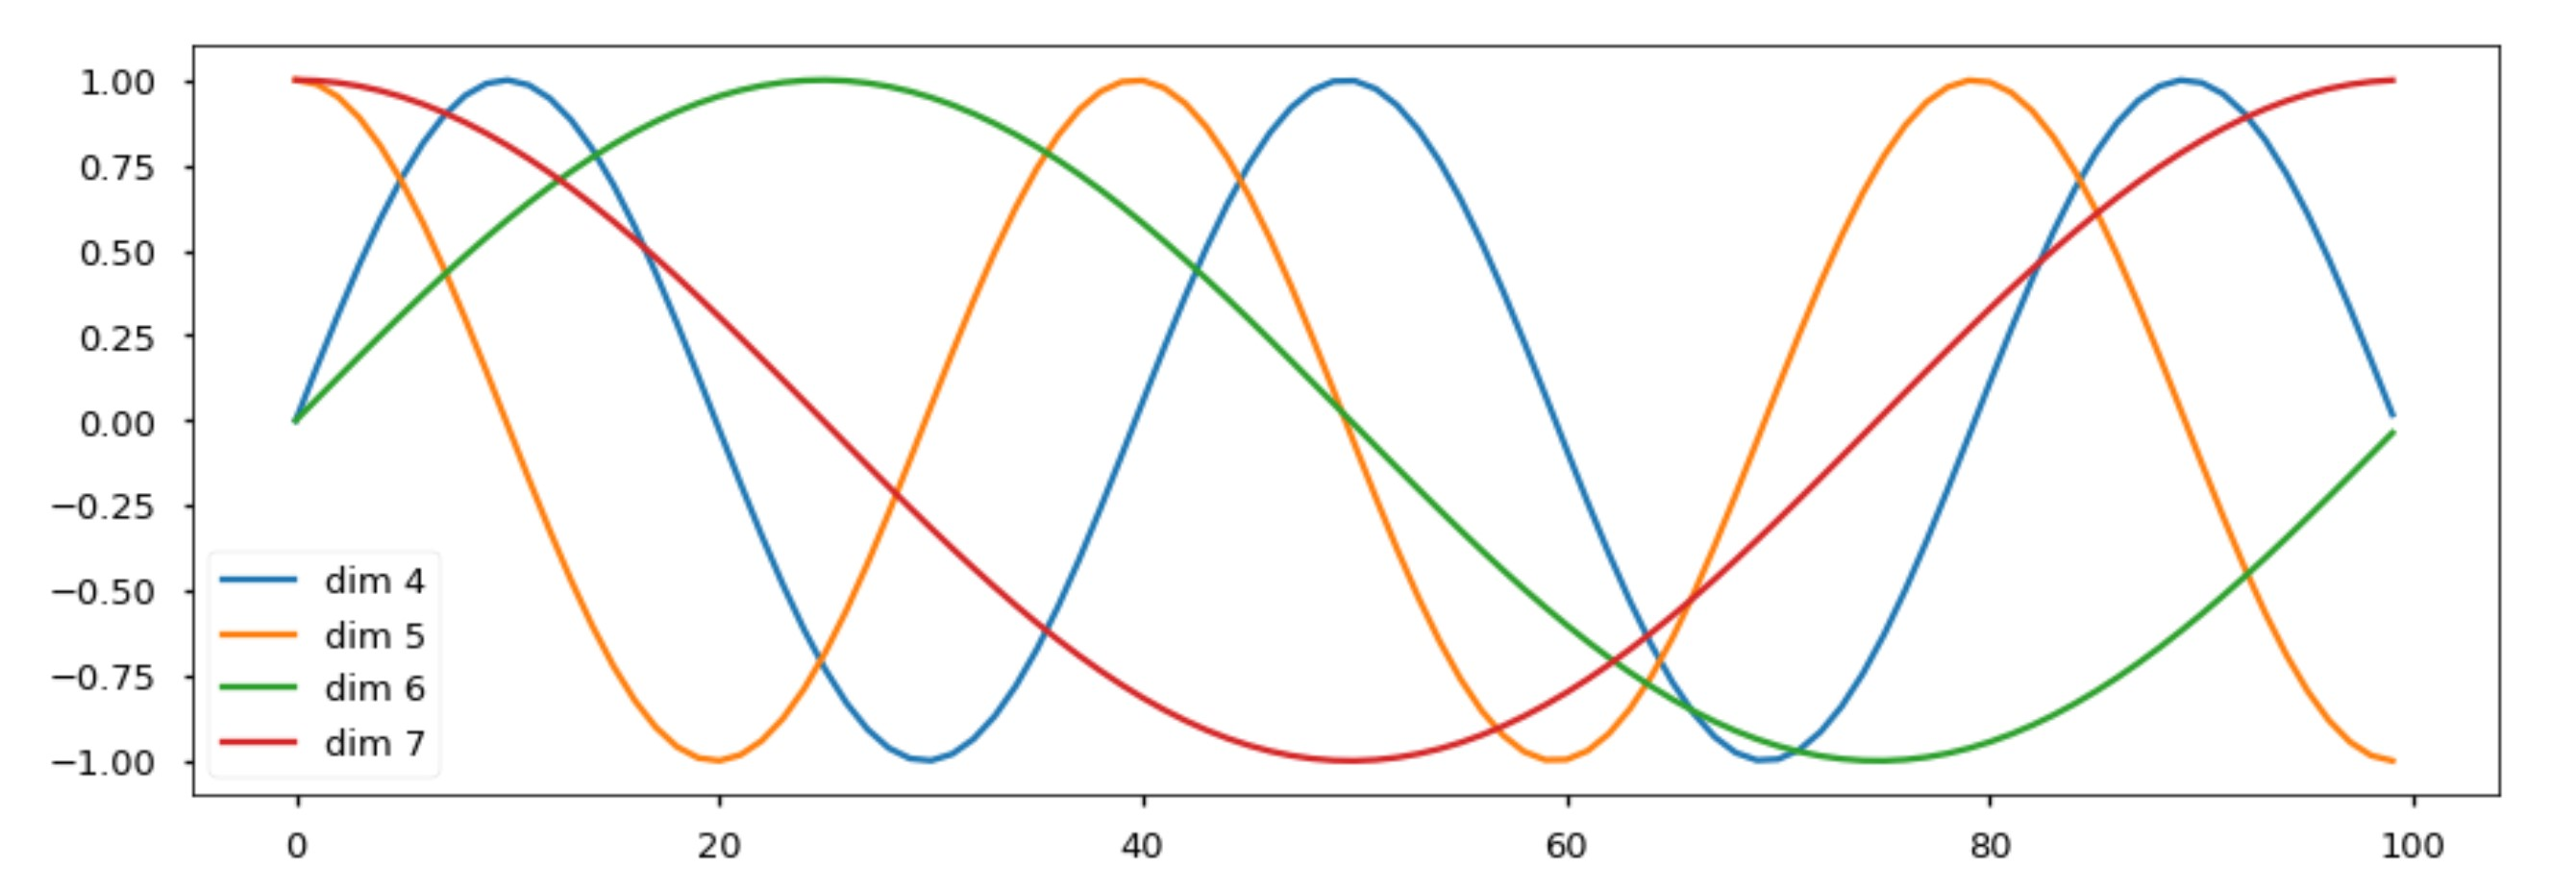
\includegraphics[width=0.7\columnwidth]{../figures/pos_enc.jpg}  
\end{center}
\caption{Positional encodings. The $x$-axis corresponds to position along the sequence ($pos$). The vertical axis is the value of $PE_{pos, i}$. Notice how each function has a different frequency, and the phase at $pos=0$ alternates between odd and even dimensions.}
\label{fig:pos_enc}
\end{figure}

\subsection{Multi-head attention}
Transformers use scaled dot product attention (Section~\ref{sec:dp-attn}), but instead of performing a single attention function with $\demb$-dimensional keys, values, and queries, they instead linearly project the queries, keys, and values $h$ times with different learnt linear projections, these are called ``\textbf{attention heads}''
\begin{equation}
\text{head}_i = \text{Attention}(QW_i^Q, KW_i^K, VW_i^V), \text{for } i = 1,...,h
\end{equation}
where $W_i^Q, W_i^K \in \mathbb{R}^{\demb \times d_k}$, $W_i^V \in \mathbb{R}^{\demb \times d_v}$ and $d_v \cdot h = d_k \cdot h = \demb$. They then concatenate each of the attention heads and apply a linear transformation
\begin{equation}
\text{MultiHead}(Q, K, V) = \text{Concat}(\text{head}_1, ..., \text{head}_h) \cdot W^O
\end{equation}
where $W^O \in \mathbb{R}^{h d_v \times \demb}$, see Fig.~\ref{fig:multi_head_attn}. Multi-head attention allows the model to jointly attend to information from different representation subspaces, at different positions. 

\begin{figure}
\begin{center}
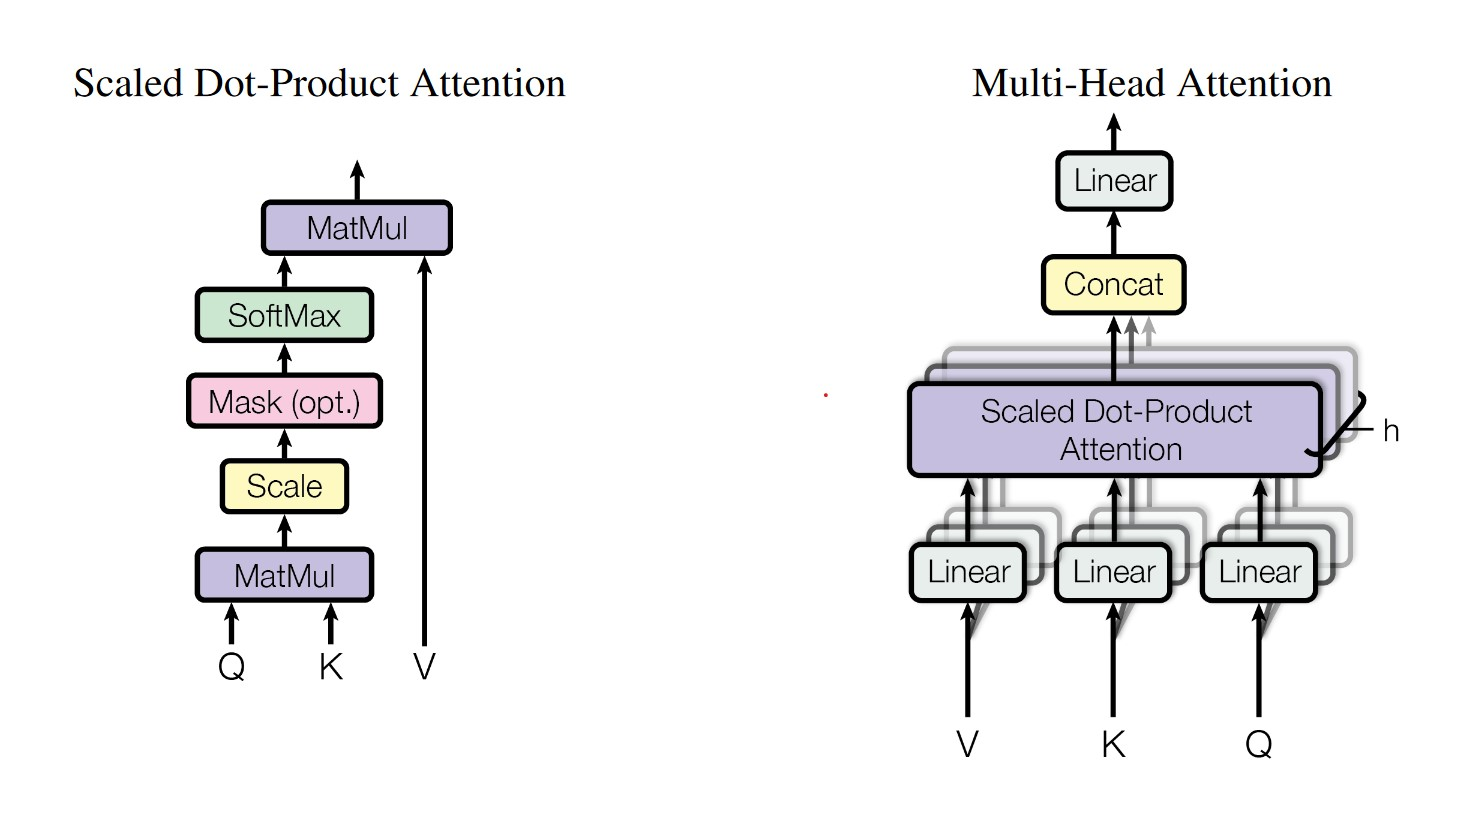
\includegraphics[width=0.7\columnwidth]{../figures/multi-head-attn.jpg}  
\end{center}
\caption{Attention mechanisms for transformers. (Left) Depiction of scaled dot-product attentions (see Section~\ref{sec:dp-attn}. Masking can be used to induce non-anticipation in the attention mechanism of the target, i.e. not using future tokens of the target to generate a prediction. Masking is also used for padding. (Right) Depiction of multi-head attention. Queries/keys/values are projected into smaller subspaces of dimension $d_k$/$d_k$/$d_v$ respectively. This is done $h$ times for all of the queries/keys/values. Scaled dot-product attention is applied to each of these attention heads. The attention heads are then concatenated together to recover the original dimension of the objects. Finally, a linear transformation is applied.}
\label{fig:multi_head_attn}
\end{figure}

\subsection{Add \& norm}
Every point in Fig.~\ref{fig:tfm} with the step ``add \& norm'' implements a layer normalization \citep{Ba16}, dropout, and then a residual connection\footnote{This is actually not what is said in the paper, but what modern implementations do because it's apparently better, \href{https://github.com/OpenNMT/OpenNMT-py/issues/770}{see here}.} \citep{He16}. This corresponds to
\begin{align}
\text{AddAndNorm}(x) &= x + \text{Dropout}(\text{Sublayer}(\text{LayerNorm}(x))) \\
\text{LayerNorm}(x) &= a \cdot \frac{x - \bar{x}}{s_x + \epsilon} + b
\end{align}
where $\bar{x}$ is the sample mean of $x$ over the final dimension (for us, $\demb$), $s_x$ is the sample standard deviation over the final dimension. $a$ and $b$ are learnable scalar parameters called the gain and bias respectively. $\text{Sublayer}(x)$ refers to the layer immediately preceding $\text{AddAndNorm}(x)$ in Fig.~\ref{fig:tfm} -- either multi-head attention or a feed-forward layer. The layer is called a residual connection because it is of the form $f(x) = x + R$, so the network is trying to learn residuals rather than $f(x)$ outright \citep{He16}.


\section{Loss functions}

\subsection{Cross entropy}
The cross-entropy $H(p,q)$ between two probability distributions $p$ and $q$ is over the same underlying set of events measures the number of bits needed to identify an event drawn from the set if a coding scheme used for the set is optimized for an estimated probability distribution $q$ rather than the true distribution $p$. It is defined as 
\begin{equation}
H(p,q) = - \sum_{x \in \mathcal{X}} p(x) \log q(x)
\end{equation}
for discrete probability distributions $p$ and $q$. The cross entropy can be written in terms of the entropy of the true distribution ($H(p)$) and the Kullback-Leibler divergence ($D_{\text{KL}}(p||q)$)
\begin{equation}
H(p,q) = H(p) + D_{\text{KL}}(p||q).
\end{equation}
[\textbf{TODO}: which will almost certainly have some sort of energetics interpretation too] 

Minimizing the cross-entropy is the same as maximizing the log-likelihood for a multinomial model (which is called a ``bag of words'' model in language modelling). We typically use $p$ as the empirical probability in the test set, and $q$ as the model predicted probability.

\subsection{Label smoothing}
Suppose that there exists a single true label $y$ over classification classes $k$. Using the same notation above for cross entropy, then for a particular training example $x$ we will have $p(k)=\delta_{k,y}$. We typically generate $q(k|x)= \text{softmax}(z_k)$ where $z_k$ is a logit. The fact that the target distribution is a Dirac delta function means that the only way to achieve the target distribution is to have $z_y \gg z_k$. This can cause: i) overfitting; ii) the model to become less adaptive, due to the gradient of $H(p,q)$ w.r.t.\ $z_k$ being bounded between -1 and 1. \cite{Szegedy16} propose replacing the label distribution $q(k|x)=\delta_{k,y}$ with
\begin{equation}
q'(k|x) = (1-\epsilon) \delta_{k,y} + \epsilon u(k)
\end{equation}
where $u(k)$ is independent of the training example $x$. They typically choose this to be the model prior, namely the discrete uniform distribution. This amounts to replacing the target with a uniformly random category with probability $\epsilon$ during training. 

% \section{Optimization}  # TODO

\newpage
\bibliography{seq.bib} 

\end{document}